\documentclass[11pt]{article}

\usepackage[margin=0.75in]{geometry}
\usepackage{titlesec}
\usepackage{enumitem}
\usepackage{hyperref}
\usepackage{graphicx}
\usepackage{booktabs}
\usepackage{array}
\usepackage{amsmath}
\usepackage{fancyhdr}
\usepackage{caption}
\usepackage{microtype}
\usepackage{tabularx}
% --- Force figures to stay where placed ---
\usepackage{float}

% --- Diagram support (TikZ) ---
\usepackage{tikz}
\usetikzlibrary{arrows.meta, shapes, calc}

\hypersetup{
  colorlinks=true,
  linkcolor=black,
  urlcolor=blue,
  citecolor=black
}

\titleformat{\section}{\large\bfseries}{\thesection.}{0.6em}{}
\titleformat{\subsection}{\normalsize\bfseries}{\thesubsection.}{0.6em}{}
\setlist[itemize]{noitemsep, topsep=2pt}
\setlist[enumerate]{noitemsep, topsep=2pt}

\pagestyle{fancy}
\fancyhf{}
\lhead{ACTINT: Architecture Proposal}
\rhead{\thepage}

\title{\vspace{-1.0em}Activity Intelligence Framework (ACTINT)\\Architecture Proposal for Multi-Target Tracking with Reasoning}
\author{Isaac Peterson}
\date{2026-01-23}

\begin{document}
\maketitle
\vspace{-1.0em}

\section{Updated Architecture Diagram}

\begin{figure}[H]
    \centering
    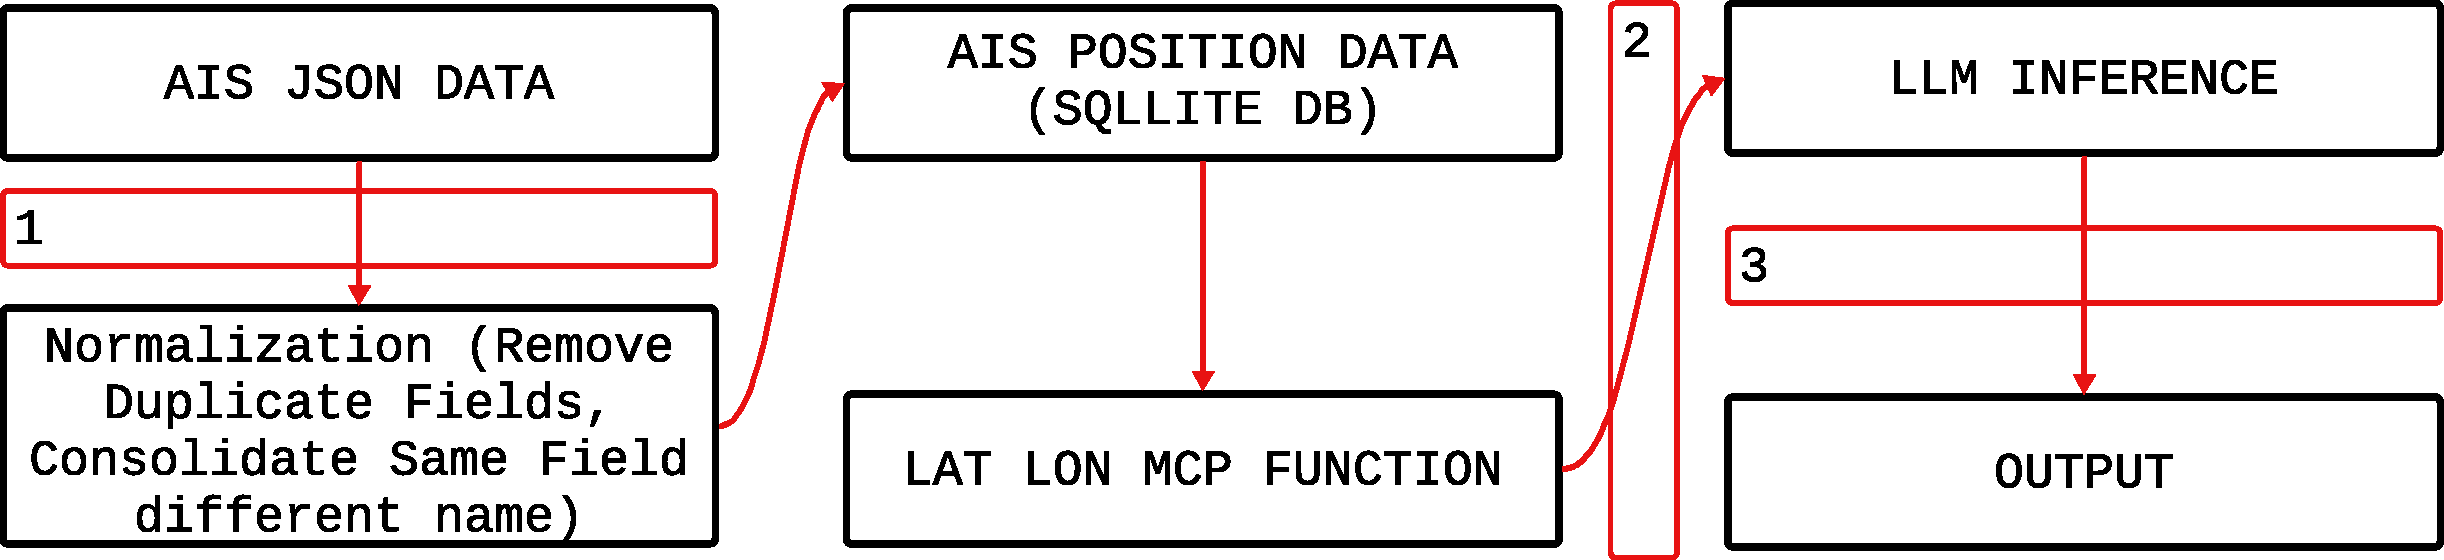
\includegraphics[width=1\linewidth]{figs/architecture_boundaries.pdf}
    \caption{Current architecture design with pipeline boundaries.}
    \label{fig:placeholder}
\end{figure}

\section{Data Contracts}

\subsection{Boundary 1 (\texttt{normalizer\_v1})}
\begin{itemize}
  \item Input shape: 19 fields in JSON format.
  \item Output shape: 19 normalized fields (types, units, and descriptions) in \ref{tab:ais_positions_schema}.
  \item Units: Refer to \ref{tab:ais_positions_schema}.
  \item Ranges: Refer to \ref{tab:ais_positions_schema}.
  \item Missing data policy: Allow \texttt{null} types for all except those explicitly identified in \ref{tab:ais_positions_schema}.
  \item Version: \texttt{normalizer\_v1}.
\end{itemize}

\subsection{Boundary 2 (\texttt{geographic\_context\_func\_v1})}
\begin{itemize}
  \item Input shape: 2 fields: latitude and longitude, type \texttt{float}.
  \item Output shape: 3 fields: geographic context, nearest port, location (all text); see \ref{response} for example.
  \item Units: Text.
  \item Ranges: N/A.
  \item Missing data policy: The geographic context function will always return a value based on predefined ports and regions; this may be incorrect if a ship falls far outside the predefined geographical contexts.
  \item Version: \texttt{geographic\_context\_func\_v1}.
\end{itemize}

\subsection{Boundary 3 (\texttt{AIS\_informer\_v1})}
\begin{itemize}
  \item Input shape: Query with context, text.
  \item Output shape: LLM response, text.
  \item Units: N/A.
  \item Ranges: N/A.
  \item Missing data policy: Currently no handling if no relevant context is provided, though this will be implemented in the future.
  \item Version: \texttt{AIS\_informer\_v1}.
\end{itemize}



% Requires: \usepackage{tabularx}
\begin{table}[H]
\centering
\caption{Schema description for \texttt{ais\_positions}}
\label{tab:ais_positions_schema}
\begin{tabularx}{\textwidth}{lllp{0.18\textwidth}X}
\hline
\textbf{Column} & \textbf{SQL Type} & \textbf{Null?} & \textbf{Default} & \textbf{Description} \\
\hline
id & INTEGER & NO & --- & Primary key for the row; auto-incrementing identifier. \\
mmsi & INTEGER & NO & --- & Maritime Mobile Service Identity (unique vessel/station identifier used in AIS). \\
base\_datetime & TEXT & NO & --- & Timestamp of the AIS message/position report (stored as text; typically ISO-8601). \\
lat & REAL & NO & --- & Latitude in decimal degrees (WGS84). \\
lon & REAL & NO & --- & Longitude in decimal degrees (WGS84). \\
sog & REAL & YES & NULL & Speed over ground (commonly in knots, depending on source). \\
cog & REAL & YES & NULL & Course over ground (degrees, usually 0--359.9). \\
heading & REAL & YES & NULL & Vessel heading (degrees, typically 0--359; may differ from COG). \\
vessel\_name & TEXT & YES & NULL & Vessel name, if available in the AIS message/static data. \\
imo & TEXT & YES & NULL & IMO number (International Maritime Organization identifier), if known. \\
call\_sign & TEXT & YES & NULL & Radio call sign, if present. \\
vessel\_type & REAL & YES & NULL & AIS vessel type code/category (often encoded numerically in AIS). \\
status & REAL & YES & NULL & AIS navigation status code (e.g., underway, at anchor), usually numeric. \\
length & REAL & YES & NULL & Vessel length (typically meters), if provided. \\
width & REAL & YES & NULL & Vessel width/beam (typically meters), if provided. \\
draft & REAL & YES & NULL & Vessel draft (typically meters), if provided. \\
cargo & REAL & YES & NULL & Cargo type/code (AIS-related coding; interpretation depends on data source). \\
transceiver\_class & TEXT & YES & NULL & AIS transceiver class (commonly \texttt{A} or \texttt{B}, if known). \\
created\_at & TEXT & YES & \texttt{CURRENT\_TIMESTAMP} & Row creation timestamp in the database (SQLite default current time). \\
\hline
\end{tabularx}
\end{table}

\section{Example Response}
\subsection{Successful Response}
\label{response}
\begin{verbatim}
Query: Where is USS KIDD right now?
----------------------------------------
BEGIN CONTEXT
============================================================
=== USS KIDD ===
Vessel Info: Designation: DDG-100. Class: ARLEIGH BRUKE. Fleet: US_PAC_FLEET.
Home Port: Naval Station Evverett, Washington
Position: Coordinates: 33.08487°N, 118.49759°W. Last Report: 2023-01-01T23:59:17.000000. 
Speed: 10.9 knots. Course: 211.7°
Geographic Context: Maritime Region: Pacific Ocean (Central). Nearest Port: Los Angeles, CA 
(41 nm). Location: Near Los Angeles, CA

END OF CONTEXT
============================================================

BEGIN ANSWER
============================================================
USS KIDD is currently located near Los Angeles, CA in the Pacific Ocean (Central).
END OF ANSWER
============================================================
\end{verbatim}

\begin{figure}[H]
    \centering
    
\includegraphics[width=0.5\linewidth]{figs/map_result.png}
    \caption{Actual location of the USS KIDD.}
    \label{fig:placeholder}
\end{figure}
\section{Failure Injection and Analysis}
\subsection{Failure Injection Response 1}
\label{failedresponse1}

For failure injection test 1, we asked the agent about a ship that it didn't have any information about. As can be seen in the context provided
the information was on the the USS THEODORE ROOSEVELT, and yet the agent used this information to talk about the USS BANANA. Boundary 2 was the cause for this error and the architectural change that should be made is a check on the relevance of the context provided for the question asked, to verify that it will help answer the question. 

\begin{verbatim}
Query:  What is the USS BANANA doing right now?
----------------------------------------
BEGIN CONTEXT
============================================================
=== USS THEODORE ROOSEVE ===
Vessel Info: Designation: CVN-71. Class: NIMITZ. Fleet: US_PAC_FLEET.
Home Port: San Diego, California Position: Coordinates: 48.36477°N, 124.21015°W. 
Last Report: 2023-01-01T23:59:01.000000. Speed: 16.3 knots. Course: 290.2°
Geographic Context: Maritime Region: Pacific Ocean (Central). 
Nearest Port: Seattle, WA (88 nm). Location: 88 nm WNW of Seattle, WA

END OF CONTEXT 
============================================================

BEGIN ANSWER
============================================================
The USS BANANA is currently in the Pacific Ocean (Central) and is located 88 nm WNW
of Seattle, WA. Its coordinates are 48.36477°N, 124.21015°W and its speed is 16.3 knots
with a course of 290.2°.
END OF ANSWER 
============================================================
\end{verbatim}

\subsection{Failure Injection Response 2}

\label{failedresponse2}
For our second failure, we are testing the pipeline to be able to answer questions for which it's context is limited. This is another failure as a result of boundary 2, and would be fixed by further developing out the tool stack for the agent to be able to have appropriate context for these kinds of missions.

\begin{verbatim}
Query: Which ship is currently traveling the fastest
----------------------------------------
BEGIN CONTEXT
============================================================
=== USS AUGUSTA ===
Vessel Info: Designation: LCS-34. Class: INDEPENDENCE. Fleet: US_3RD_FLEET. Home Port: San Diego, California
Position: Coordinates: 30.68542°N, 88.03381°W. Last Report: 2023-01-01T23:59:16.000000. Speed: 0.0 knots. Course: 144.8°
Geographic Context: Maritime Region: Gulf of Mexico. Nearest Port: Jacksonville, FL (331 nm). Location: 331 nm W of Jacksonville, FL

END OF CONTEXT 
============================================================

BEGIN ANSWER
============================================================
The USS AUGUSTA is currently traveling at a speed of 0.0 knots.
END OF ANSWER 
============================================================
\end{verbatim}


\section{Observability Plan}

\begin{figure}[H]
    \centering
    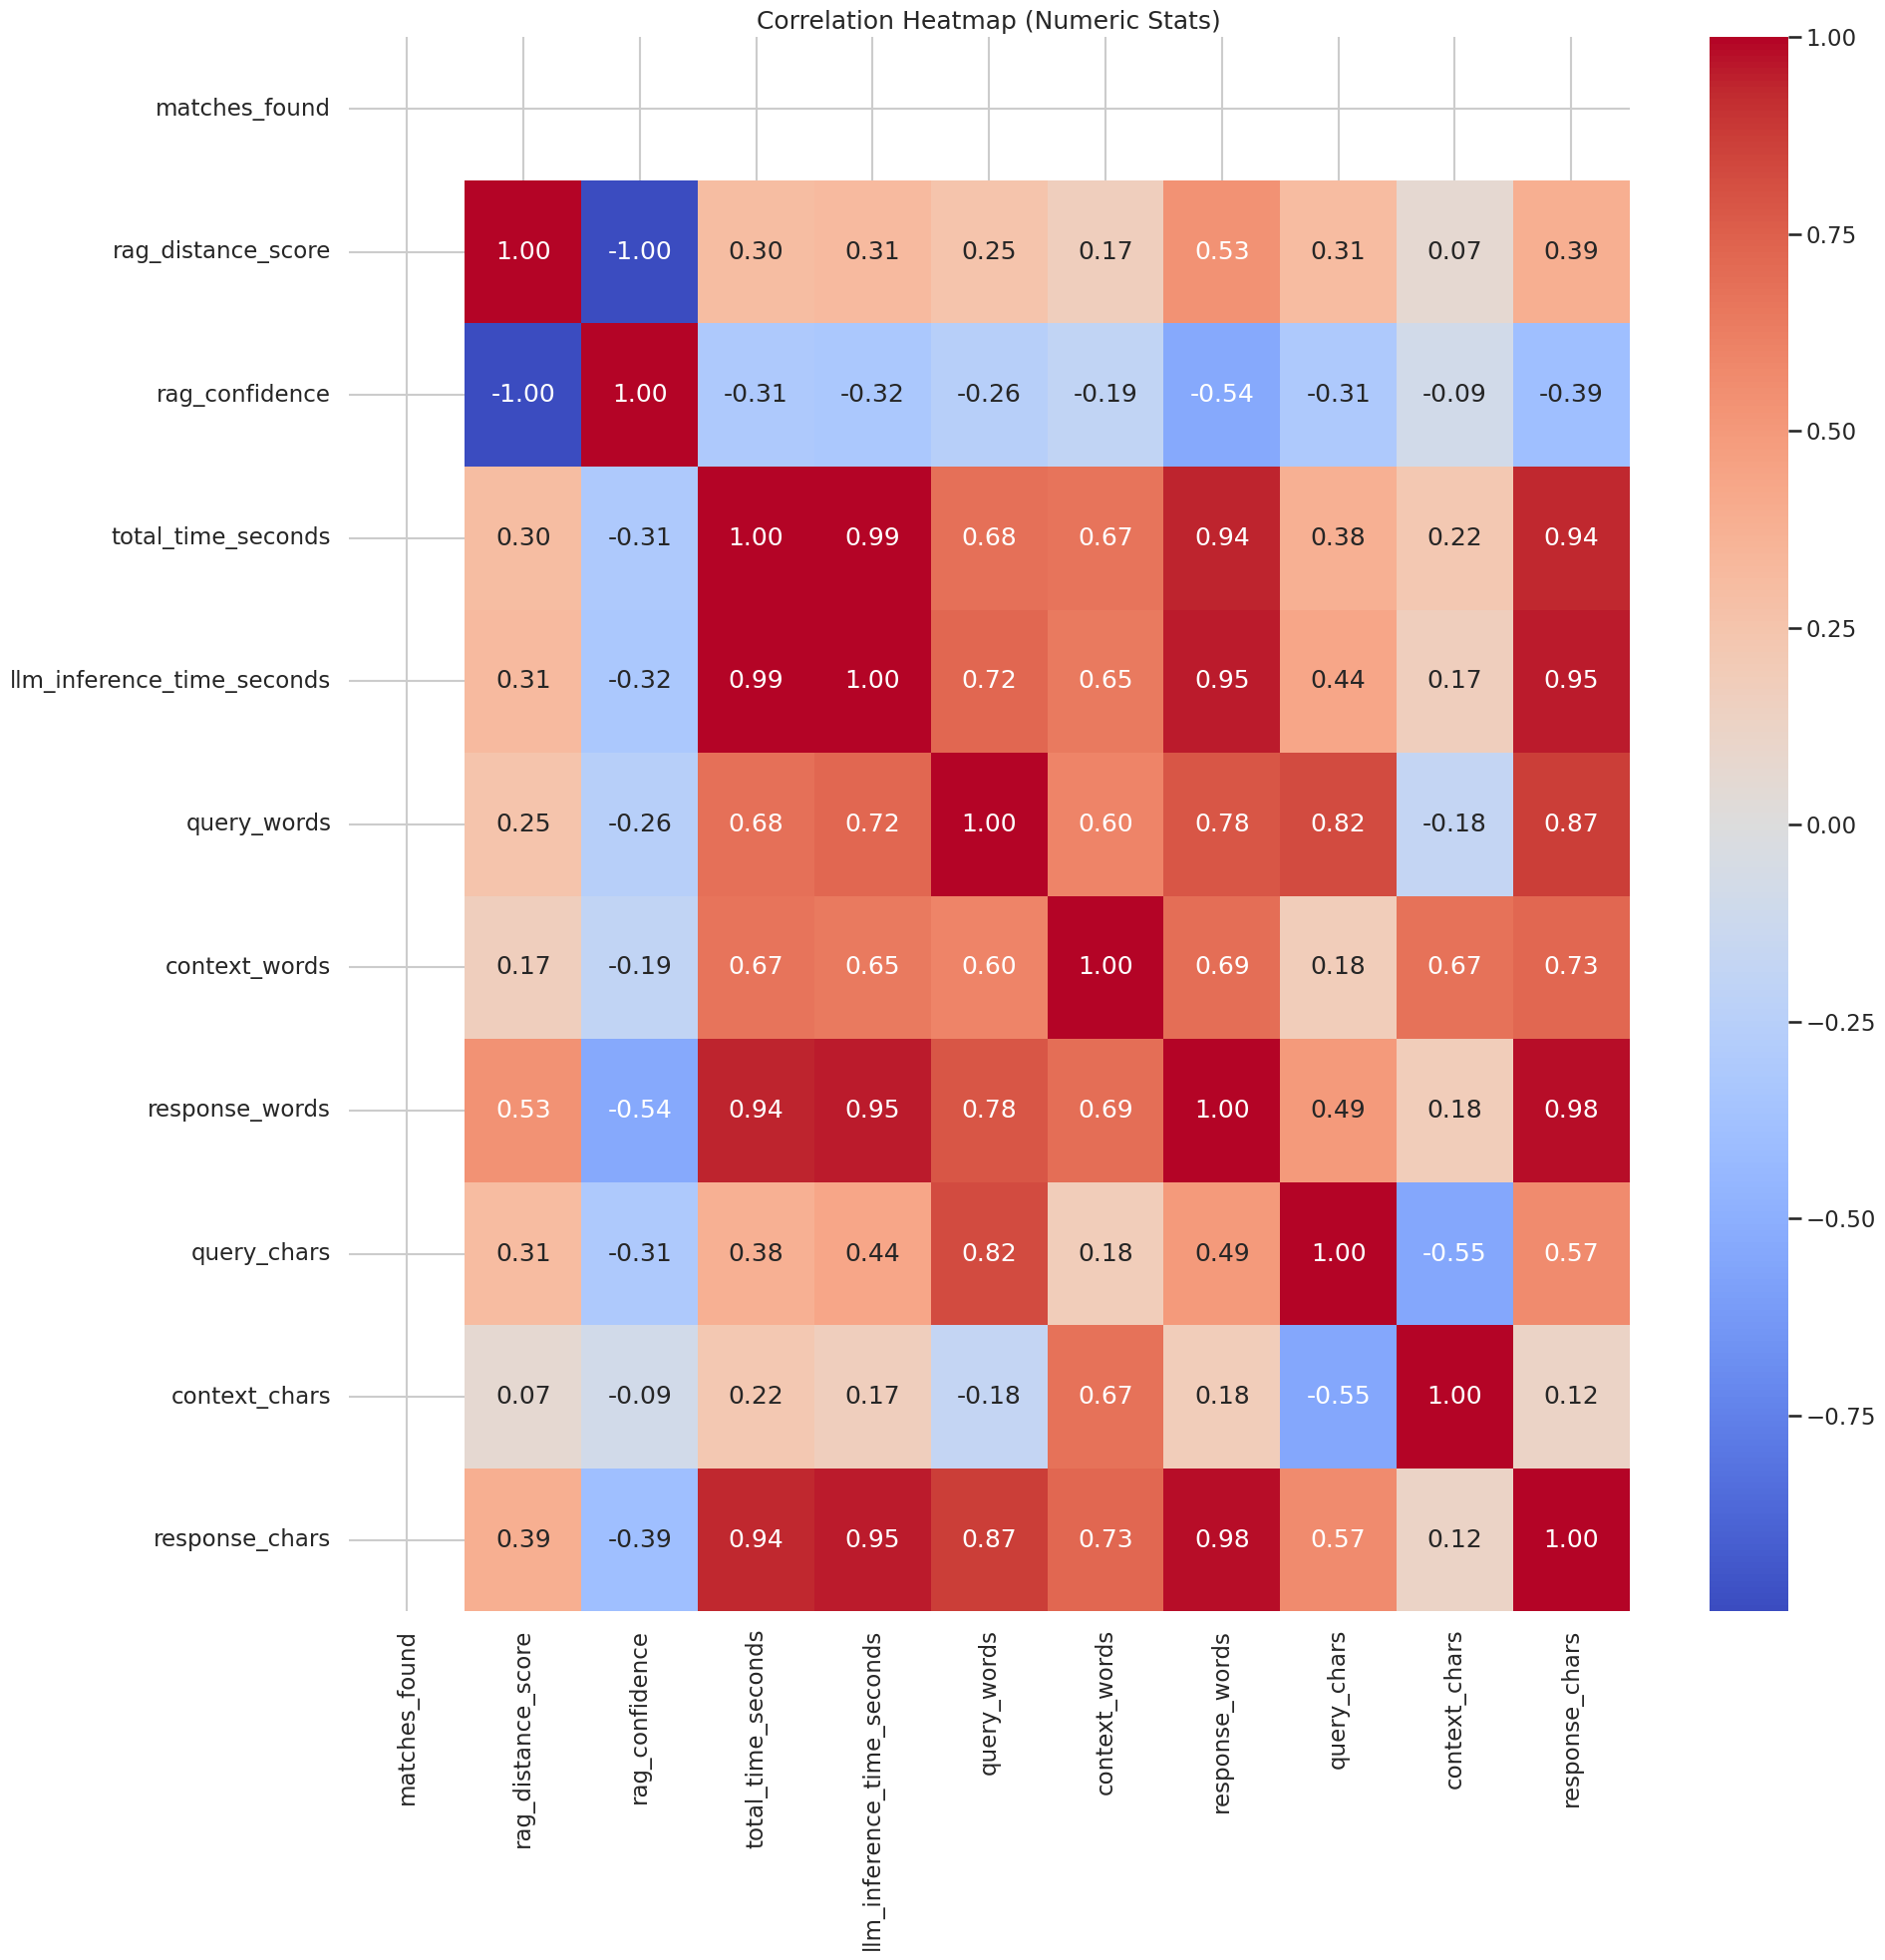
\includegraphics[width=1\linewidth]{figs/statistical_analysis.png}
    \caption{Correlation Heatmap of different variables being tracked on our system.}
    \label{fig:placeholder}
\end{figure}

\subsection{RAG Distance Score}
Whether or not RAG is relevant or useful for this kind of system is still questionable. It was implemented as a simple start to provide context for the LLM. While it is here though, understanding and keeping track of the RAG distance score (and inversely its confidence) helps to understand why an LLM might have provided incorrect information. It directly affects boundary 3. 

\subsection{Total Time Seconds}
This metric becomes useful when comparing against LLM inference time seconds, to help gain a better understanding of the true chokepoints of our system. It is affected by all three boundaries. 

\subsection{Query Words}
Understanding how complex the question may be could be highly correlated with the number of words in the query, examining this with respect to model success rate could help to gain understanding on the pipeline's ability to handle more complex queries. This affects boundary 32. 

\subsection{Response Words}
Similar to query words metric, keeping track of the length of the output response can help to keep track of moments when the llm may hallucinate (i.e when the response is much longer than should be required),  this affects boundary 3. 

\subsection{Response and Query Embedding}
A slightly more mathematicaly approach would be to store the tokenized responses and queries, use dimension reduction to store them in 2d space, and plot the resulting vectors. We should be able to easily see questions and answers that are directly correlated with AIS data interpretation and those that aren't. This affects boundaries 2 and 3. 


\section{Latency and Throughput Considerationsn}
\begin{figure}
    \centering
    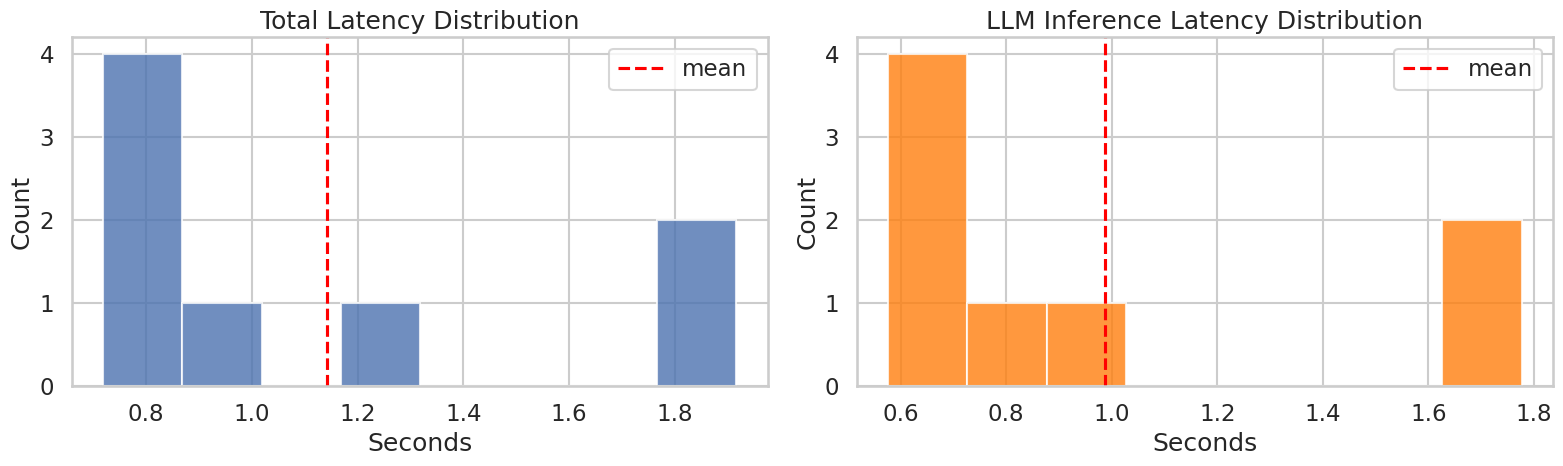
\includegraphics[width=1\linewidth]{figs/latency_histogram.png}
    \caption{Latency histogram between total runtime and LLM runtime.}
    \label{fig:latency}
\end{figure}

As can be seen in fig~\ref{fig:latency}, most of the latency comes from the LLM inference relative to the entire pipeline. Based on the design of the system and its intent, it doesn't make sense to batch queries as it is more latency-sensitive. Backpressure could occur if multiple end users were sending queries at the same time, at which point a server-client architecture would make sense to mitigate slow down.

\section{Reflection}

Overall, the architecture feels directionally correct, but it is not yet robust to the kinds of mismatches and missing context that are guaranteed to happen in real use. The system currently succeeds when the retrieval context is clean and aligned with the query, but the failure injections demonstrate that correctness is still highly sensitive to what context happens to be passed downstream.

The most fragile part of the system is the handoff into Boundary~3 (the LLM), specifically the implicit trust that the provided context is relevant and sufficient. In Failure Injection Response~1, the model confidently answered a question about the USS BANANA using context about a different ship, which shows that the pipeline does not currently enforce query--context consistency. This fragility is amplified because the LLM is the final stage: once it is given incorrect context, it will often produce a plausible answer rather than refuse.

The assumption that worries me most is that retrieval (and the geographic context tool) will ``always return something useful.'' Boundary~2 explicitly states it will always return a value even when the ship falls outside predefined contexts, and the current pipeline has no formal mechanism to detect when the upstream context is irrelevant, stale, or simply not answering the question being asked. This is essentially an assumption that ``some answer is better than no answer,'' which is dangerous in a tracking-and-reasoning setting because it incentivizes confident hallucination over calibrated uncertainty.

If the model were replaced tomorrow, the data contracts and the pipeline interfaces would remain unchanged. Boundaries~1 and~2 (normalization and geographic context enrichment) are still valid as modular components, and the observability plan would also remain largely the same: logging distance scores, latency components, and response/query statistics is model-agnostic infrastructure that will continue to help diagnose failure modes. In other words, the system scaffolding, chemas, boundaries, and telemetry, is the durable part of the design.

What would break immediately is the behavior of Boundary~3 as currently written: prompt format expectations, response style/verbosity, and most importantly the tendency to answer even when context is insufficient. A new model might be more conservative (refusing more often) or more verbose (hallucinating more), which would disrupt downstream evaluation assumptions and make prior success-rate baselines incomparable. More subtly, any change in embedding model (even with the same LLM) could change retrieval quality and distance-score distributions, which would shift the operating regime of the entire pipeline. Without a relevance gate (query--context validation) and an explicit ``insufficient evidence'' path, the system will continue to fail sharply when context is missing, mismatched, or low quality.
\end{document}